\chapter{The Metrics Pipeline}
\label{ch:metrics}

A benchmark is only as good as the data it produces.  This chapter describes
the \emph{metrics pipeline}---the system of collectors, aggregators, and
schemas that turns raw sensor readings, packet counters, and timing samples
into the structured JSON files that later feed the analysis dashboard.

\begin{keyinsight}
The pipeline follows a three-stage architecture:
\textbf{(1)}~\emph{Collectors} read hardware sensors and software counters.
\textbf{(2)}~\emph{Aggregator} merges per-collector data into a single typed
object.
\textbf{(3)}~\emph{Persistence} writes the object to JSON and JSONL for
offline analysis.
Think of it as a factory assembly line: raw materials (sensor readings) enter
at one end, and a finished product (a complete JSON record) exits the other.
\end{keyinsight}

% ============================================================
\section{The 18-Category Schema}
\label{sec:metrics-schema}

Every suite benchmark produces a single \texttt{ComprehensiveSuiteMetrics}
object, defined in \texttt{core/metrics\_schema.py}.  This object contains
18~nested dataclasses, labelled A through~R.  Table~\ref{tab:metrics-18cat}
lists every category, its purpose, and its approximate field count.

\begin{table}[htbp]
\centering
\caption{The 18-category metrics schema}
\label{tab:metrics-18cat}
\begin{tabular}{@{}c l p{5.2cm} c@{}}
\toprule
\textbf{Cat} & \textbf{Name} & \textbf{Purpose} & \textbf{Fields} \\
\midrule
A & Run \& Context           & Run ID, git hash, hostnames, IPs, clock offset & 20 \\
B & Suite Crypto Identity    & KEM, SIG, AEAD algorithms and NIST level & 8 \\
C & Suite Lifecycle Timeline & Selection, activation, deactivation timestamps & 5 \\
D & Handshake Metrics        & Total duration, success, failure reason & 7 \\
E & Crypto Primitive Breakdown & Per-primitive timing (ns) and artifact sizes (bytes) & 14 \\
F & Rekey Metrics            & Attempts, successes, failures, intervals & 7 \\
G & Data Plane (Proxy)       & Throughput, packet counts, drops, AEAD timing & 20+ \\
H & Latency \& Jitter        & One-way latency, RTT, jitter (avg, P95) & 12 \\
I & MAVProxy Drone           & TX/RX PPS, message counts, heartbeat, seq gaps & 15 \\
J & MAVProxy GCS             & Validation subset: message count, seq gap count & 2 \\
K & MAVLink Integrity        & CRC errors, decode errors, drops, duplicates & 9 \\
L & Flight Controller        & FC mode, armed state, battery, CPU, sensors & 10 \\
M & Control Plane            & Scheduler action, policy name, suite index & 7 \\
N & System Resources (Drone) & CPU, memory, temperature, load averages & 12 \\
O & System Resources (GCS)   & Retained for schema compatibility (not collected) & 11 \\
P & Power \& Energy          & Voltage, current, power, energy per handshake & 8 \\
Q & Observability            & Sample counts, collection timestamps & 5 \\
R & Validation \& Integrity  & Pass/fail verdict, per-metric status map & 5 \\
\bottomrule
\end{tabular}
\end{table}

\begin{designdecision}
Category~O (GCS system resources) is \emph{retained in the schema but no
longer collected}.  The GCS is a non-constrained observer---its CPU and memory
do not influence policy decisions, suite ranking, or cryptographic selection.
Collecting them added overhead without policy value.  The fields remain at
\texttt{None} for forward compatibility.
\end{designdecision}

\subsection{Schema Design Principles}

\begin{enumerate}
  \item \textbf{Typed dataclasses}: Every field has an explicit Python type
        (\texttt{Optional[float]}, \texttt{Optional[int]}, etc.).  This
        catches type errors at development time and makes JSON serialisation
        straightforward via \texttt{dataclasses.asdict()}.

  \item \textbf{Optional fields}: Nearly every field is
        \texttt{Optional[...]}, defaulting to \texttt{None}.  This means
        a partially-filled record is still valid---essential when some
        collectors fail (e.g.\ power monitoring is unavailable on the dev
        laptop).

  \item \textbf{Dual serialisation}: The \texttt{ComprehensiveSuiteMetrics}
        class provides both \texttt{to\_dict()} / \texttt{to\_json()} for
        export and \texttt{from\_dict()} / \texttt{from\_json()} for import,
        enabling round-trip fidelity.

  \item \textbf{Flat JSON output}: When serialised, the 18 categories become
        top-level keys (\texttt{run\_context}, \texttt{crypto\_identity},
        \ldots, \texttt{validation}), each containing a flat dictionary of
        fields.  This structure is directly consumable by the dashboard
        backend.
\end{enumerate}

% ============================================================
\section{Collectors}
\label{sec:metrics-collectors}

Collectors are the lowest layer of the pipeline.  Each one reads a specific
data source and returns a plain dictionary.

\subsection{EnvironmentCollector}

Captures static context about the run environment---information that does not
change during the benchmark:

\begin{itemize}
  \item Hostname, platform, Python version
  \item Kernel version (via \texttt{platform.platform()})
  \item Git commit hash and dirty flag (via \texttt{git rev-parse} and
        \texttt{git status})
  \item \texttt{liboqs} version (detected from the installed package)
  \item Conda or virtualenv environment name
  \item IP address (resolved via socket)
  \item Wall-clock and monotonic start timestamps
\end{itemize}

This collector runs once at suite start and populates Category~A.

\subsection{SystemCollector}

Samples live system resource telemetry using \texttt{psutil}:

\begin{itemize}
  \item CPU usage percent (with rolling min/max/avg statistics)
  \item CPU frequency (MHz)
  \item Process RSS and VMS memory (MB)
  \item Thread count
  \item System uptime, load averages (1/5/15~min on Linux)
  \item Temperature and thermal throttling (on Raspberry Pi, via
        \texttt{vcgencmd measure\_temp})
\end{itemize}

The aggregator runs this collector in a background thread at 0.5\,Hz during
each suite, then computes summary statistics at suite end.  Results populate
Categories~N (drone) and~O (GCS, deprecated).

\subsection{PowerCollector}
\label{sec:metrics-power}

The power collector auto-detects the available backend:

\begin{description}
  \item[INA219] An external current-sense amplifier connected via I\textsuperscript{2}C.
        Provides high-frequency sampling (up to $\sim 1{,}100$\,Hz on the
        ``highspeed'' ADC profile).
  \item[RPi5 hwmon] The Raspberry Pi~5's on-board PMIC exposes voltage,
        current, and power via the Linux \texttt{sysfs/hwmon} interface.
        No external hardware required.
  \item[None] On platforms without power monitoring hardware (e.g.\ the
        development laptop), the collector returns empty data.
\end{description}

Results populate Category~P.

\subsection{NetworkCollector}

Reads NIC-level I/O counters from \texttt{psutil.net\_io\_counters()}:
RX/TX bytes, packets, errors, and drops.  By computing deltas between
consecutive calls, it derives instantaneous throughput rates in Mbps.

\subsection{MavLinkMetricsCollector}
\label{sec:metrics-mavlink}

This is the most complex collector.  It sniffs live MAVLink traffic from
a \texttt{pymavlink} UDP connection and tracks dozens of metrics in real
time.

\subsubsection{Architecture}

The collector opens a \texttt{udpin:} socket on a designated sniff port
(typically 14552 on GCS, 47005 on drone) and spawns a daemon thread that
calls \texttt{conn.recv\_match()} in a tight loop.  Each received message is
dispatched by type to specialised handlers.

\subsubsection{Tracked Metrics}

\begin{table}[htbp]
\centering
\caption{MAVLink collector metric groups}
\label{tab:metrics-mavlink-groups}
\begin{tabular}{@{}l p{7cm}@{}}
\toprule
\textbf{Group} & \textbf{Metrics} \\
\midrule
Message rates   & TX/RX packets per second, stream rate Hz \\
Message counts  & Total sent/received, per-type histogram \\
Heartbeat       & Count, expected, loss count, interval (ms), armed state,
                  flight mode \\
Sequence integrity & Gap count, duplicates, out-of-order count \\
Command latency & Commands sent, ACKs received, avg \& P95 ACK latency (ms) \\
One-way latency & Derived from \texttt{time\_usec} in timestamped messages
                  (avg, P95, jitter, validity flag + reason) \\
Round-trip time & From COMMAND\_LONG $\to$ COMMAND\_ACK (avg, P95) \\
Errors          & CRC errors, decode errors, message drops \\
Flight controller & Mode, armed, battery V/A/\%, CPU load, sensor health \\
\bottomrule
\end{tabular}
\end{table}

\subsubsection{One-Way Latency Estimation}

\begin{analogy}
Imagine you and a friend each have a stopwatch.  Your friend stamps each
letter with the time on \emph{her} stopwatch.  When the letter arrives, you
read the stamp and compare it to \emph{your} stopwatch.  The difference is the
one-way latency---but only if both stopwatches are synchronised (or at least
if you know their offset).
\end{analogy}

MAVLink messages like \texttt{GLOBAL\_POSITION\_INT} and \texttt{ATTITUDE}
carry a \texttt{time\_boot\_ms} timestamp from the flight controller's boot
clock.  The collector establishes a \texttt{boot\_to\_unix\_offset\_s} by
comparing the first such timestamp against the local wall clock.  Subsequent
messages use this offset to estimate one-way latency:

\[
\text{latency} = t_{\text{receive}} - (t_{\text{boot\_ms}} / 1000 +
\text{offset})
\]

If fewer than 5~samples are collected, or if no timestamped messages arrive
at all, the latency is marked invalid with a reason string such as
\texttt{"missing\_system\_time\_reference"} or
\texttt{"insufficient\_samples"}.

\subsubsection{Sequence Gap Detection}

Every MAVLink message carries an 8-bit sequence number per system ID.
The collector tracks the last sequence number for each system ID and
counts:
\begin{itemize}
  \item \textbf{Gaps}: expected $\neq$ received (messages lost in transit).
  \item \textbf{Duplicates}: same sequence number twice.
  \item \textbf{Out-of-order}: lower sequence number than expected (but not
        a wraparound).
\end{itemize}

These populate Category~K (MAVLink Integrity).

% ============================================================
\section{The INA219 Power Monitor}
\label{sec:metrics-ina219}

The INA219 is a Texas Instruments current-sense amplifier that measures both
the voltage across and the current through a shunt resistor.  It communicates
over I\textsuperscript{2}C.

\begin{figure}[htbp]
\centering
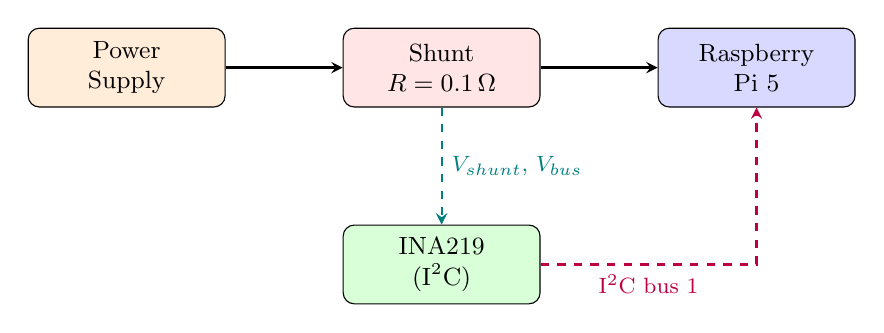
\begin{tikzpicture}[
    comp/.style={draw, rounded corners, minimum width=2.5cm,
                 minimum height=1cm, font=\small, align=center},
    arr/.style={->, >=stealth, thick}
  ]
  \node[comp, fill=orange!15] (psu) at (0,0) {Power\\Supply};
  \node[comp, fill=red!10] (shunt) at (4,0) {Shunt\\$R=0.1\,\Omega$};
  \node[comp, fill=blue!15] (rpi) at (8,0) {Raspberry\\Pi 5};
  \node[comp, fill=green!15] (ina) at (4,-2.5) {INA219\\(I\textsuperscript{2}C)};

  \draw[arr] (psu) -- (shunt);
  \draw[arr] (shunt) -- (rpi);
  \draw[arr, dashed, color=teal] (shunt.south) -- (ina.north)
    node[midway, right, font=\footnotesize] {$V_{\text{shunt}}$, $V_{\text{bus}}$};
  \draw[arr, dashed, color=purple] (ina.east) -| (rpi.south)
    node[near start, below, font=\footnotesize] {I\textsuperscript{2}C bus 1};
\end{tikzpicture}
\caption{INA219 measurement topology.  The sensor sits in-line between the
power supply and the Pi, measuring the voltage drop across the shunt resistor.}
\label{fig:metrics-ina219}
\end{figure}

\subsection{Register-Level Access}

Rather than using a high-level library, the codebase accesses INA219 registers
directly via \texttt{smbus2}:

\begin{itemize}
  \item \textbf{Configuration register} (0x00): Sets bus voltage range
        (32\,V), PGA gain ($\pm 320$\,mV), and ADC resolution.
  \item \textbf{Shunt voltage register} (0x01): Raw 16-bit value;
        $V_{\text{shunt}} = \text{raw} \times 10\,\mu\text{V}$.
  \item \textbf{Bus voltage register} (0x02): Raw 16-bit value shifted
        right by 3; $V_{\text{bus}} = \text{raw} \times 4\,\text{mV}$.
\end{itemize}

Current is computed via Ohm's law:
\[
I = \frac{V_{\text{shunt}}}{R_{\text{shunt}}}
\qquad
P = V_{\text{bus}} \times I
\]

\subsection{ADC Profiles}

The INA219 ADC resolution and averaging mode control the trade-off between
sample rate and precision:

\begin{table}[htbp]
\centering
\caption{INA219 ADC profiles}
\label{tab:metrics-adc}
\begin{tabular}{@{}l c c l@{}}
\toprule
\textbf{Profile} & \textbf{Effective Hz} & \textbf{Settle ($\mu$s)} & \textbf{Use case} \\
\midrule
highspeed  & $\sim 1{,}100$ & 400  & Handshake energy bursts \\
balanced   & $\sim 900$     & 1000 & General benchmarking \\
precision  & $\sim 450$     & 2000 & Long-term power profiling \\
\bottomrule
\end{tabular}
\end{table}

\subsection{Capture and Energy Integration}

The \texttt{capture(label, duration\_s)} method runs a timed sampling loop:

\begin{enumerate}
  \item Allocate a CSV file in the output directory.
  \item Loop for \texttt{duration\_s} seconds at \texttt{sample\_hz}, using
        \texttt{time.perf\_counter\_ns()} for tick-based scheduling.
  \item On each tick: read shunt voltage, compute current, read bus voltage,
        compute power, write a row to CSV.
  \item After the loop: compute summary statistics (average V/I/P, peak P,
        total energy via trapezoidal integration).
  \item Return a \texttt{PowerSummary} dataclass.
\end{enumerate}

Energy is computed as:
\[
E = \sum_{i=1}^{N-1} \frac{P_i + P_{i+1}}{2} \cdot \Delta t_i
\]

where $\Delta t_i$ is the time between consecutive samples.

\subsection{RPi5 hwmon Backend}

The Raspberry Pi~5's on-board PMIC (Power Management IC) exposes power
telemetry via the Linux \texttt{sysfs/hwmon} filesystem.  The
\texttt{Rpi5HwmonPowerMonitor} class auto-discovers the correct hwmon
directory by scanning for known chip names (e.g.\ \texttt{rpi\_volt}), then
reads:

\begin{itemize}
  \item \texttt{in0\_input} or \texttt{voltage0\_input} for voltage (mV)
  \item \texttt{curr0\_input} or \texttt{current0\_input} for current (mA)
  \item \texttt{power0\_input} for power (if available)
\end{itemize}

Scale factors convert raw sysfs values to SI units.  The capture and
\texttt{iter\_samples} methods have identical signatures to the INA219
monitor, making the two backends interchangeable.

\subsection{Sign Resolution}

Current direction depends on how the shunt resistor is wired.  The
\texttt{\_resolve\_sign()} method reads a burst of shunt voltage samples and
checks the median:

\begin{itemize}
  \item If positive: sign factor $= +1$.
  \item If negative: sign factor $= -1$.
  \item If configured as ``auto'': uses the median's sign.
\end{itemize}

This ensures that current is always reported as a positive number regardless
of wiring orientation.

% ============================================================
\section{The Metrics Aggregator}
\label{sec:metrics-aggregator}

The \texttt{MetricsAggregator} class (in \texttt{core/metrics\_aggregator.py})
is the central orchestrator that wires collectors to schema categories.  It
runs on both GCS and drone, with role-specific logic.

\subsection{Lifecycle}

\begin{enumerate}
  \item \textbf{Initialisation}: Detect role (drone or GCS), create
        collectors (environment, system, network, power on drone, MAVLink on
        both sides).
  \item \textbf{\texttt{start\_suite(suite\_id, suite\_config)}}:
    \begin{itemize}
      \item Create a fresh \texttt{ComprehensiveSuiteMetrics} object.
      \item Populate Categories~A (run context) and~B (crypto identity)
            from the environment collector and suite configuration.
      \item Record suite selection time (Category~C).
      \item Start the MAVLink collector's sniffing thread.
      \item Start background system-metric sampling.
    \end{itemize}
  \item \textbf{\texttt{record\_handshake\_start()} /
        \texttt{record\_handshake\_end()}}:
        Populate Category~D with handshake timing.
  \item \textbf{\texttt{record\_crypto\_primitives(metrics)}}:
        Populate Category~E from the handshake metrics dictionary.
  \item \textbf{\texttt{record\_data\_plane\_metrics(counters)}}:
        Populate Category~G from proxy status-file counters.
  \item \textbf{\texttt{record\_control\_plane\_metrics(\ldots)}}:
        Populate Category~M with scheduler state.
  \item \textbf{\texttt{finalize\_suite(merge\_from=None)}}:
    \begin{itemize}
      \item Stop background collectors.
      \item Compute summary statistics for system metrics (avg, peak CPU).
      \item Pull MAVLink metrics (populates Categories~H, I, J, K, L).
      \item Pull power metrics (Category~P).
      \item If \texttt{merge\_from} is provided (GCS metrics dict from the
            control channel), merge it into the object.
      \item Compute validation verdict (Category~R): check that MAVLink
            messages were received, latency is valid, and data-plane counters
            are non-zero.
      \item Return the completed \texttt{ComprehensiveSuiteMetrics} object.
    \end{itemize}
  \item \textbf{\texttt{save\_suite\_metrics(metrics)}}:
        Write the object to a JSON file in the output directory, named
        \texttt{\{timestamp\}\_\{suite\_id\}\_\{role\}.json}.
\end{enumerate}

\subsection{Cross-Side Metric Merging}

The drone is the authority for the final combined record.  When the GCS
responds to a \texttt{stop\_suite} command, it includes a
\texttt{metrics\_export} dictionary containing its aggregator's data.  The
drone's aggregator receives this via the \texttt{merge\_from} parameter of
\texttt{finalize\_suite()} and copies GCS-specific fields (MAVLink validation
counts, system metrics, latency/jitter from the GCS perspective) into the
combined object.

\begin{figure}[htbp]
\centering
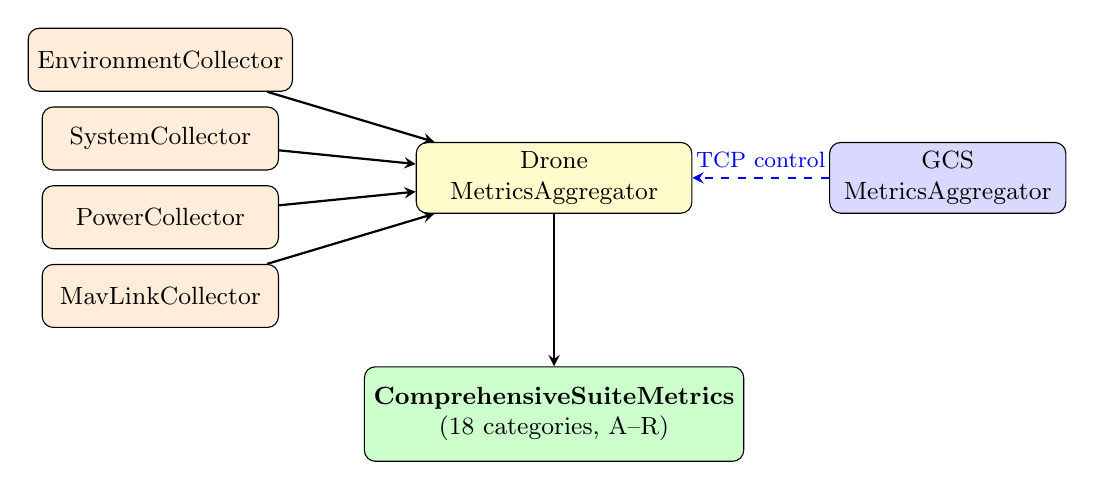
\begin{tikzpicture}[
    box/.style={draw, rounded corners, minimum width=3cm,
                minimum height=0.8cm, font=\small, align=center},
    arr/.style={->, >=stealth, thick}
  ]
  % Drone side
  \node[box, fill=orange!15] (denv) at (0,3) {EnvironmentCollector};
  \node[box, fill=orange!15] (dsys) at (0,2) {SystemCollector};
  \node[box, fill=orange!15] (dpow) at (0,1) {PowerCollector};
  \node[box, fill=orange!15] (dmav) at (0,0) {MavLinkCollector};

  \node[box, fill=yellow!20, minimum width=3.5cm] (dagg) at (5,1.5)
    {Drone\\MetricsAggregator};

  % GCS side
  \node[box, fill=blue!15] (gcs) at (10,1.5) {GCS\\MetricsAggregator};

  % Final
  \node[box, fill=green!20, minimum width=4cm, minimum height=1.2cm] (out)
    at (5,-1.5) {\textbf{ComprehensiveSuiteMetrics}\\(18 categories, A--R)};

  \draw[arr] (denv) -- (dagg);
  \draw[arr] (dsys) -- (dagg);
  \draw[arr] (dpow) -- (dagg);
  \draw[arr] (dmav) -- (dagg);
  \draw[arr, dashed, color=blue] (gcs) -- node[above, font=\footnotesize]
    {TCP control} (dagg);
  \draw[arr] (dagg) -- (out);
\end{tikzpicture}
\caption{Metric flow: four drone-side collectors and the GCS aggregator
merge into a single ComprehensiveSuiteMetrics object.}
\label{fig:metrics-flow}
\end{figure}

\subsection{Validation Verdict (Category~R)}

After all metrics are collected, the aggregator computes a pass/fail verdict:

\begin{enumerate}
  \item \textbf{MAVLink message check}: If
        \texttt{mavproxy\_drone\_total\_msgs\_received} is zero or null,
        mark \texttt{mavlink\_no\_messages}.
  \item \textbf{Latency validity check}: If neither one-way latency nor RTT
        is valid, and the reason is \emph{not} structural (e.g.\
        \texttt{missing\_system\_time\_reference}), mark
        \texttt{mavlink\_latency\_invalid}.
  \item \textbf{Data-plane check}: If both \texttt{packets\_sent} and
        \texttt{packets\_received} are zero, mark
        \texttt{data\_plane\_no\_traffic}.
  \item If any check fails: \texttt{benchmark\_pass\_fail} $\gets$
        \texttt{"FAIL"}, and the corresponding reason is recorded in the
        \texttt{metric\_status} dictionary.
\end{enumerate}

% ============================================================
\section{The RobustLogger}
\label{sec:metrics-robust}

Benchmarks can crash mid-suite---the flight controller may reboot, a proxy may
segfault, or the Raspberry Pi may lose power.  If metrics are only written at
suite end, a crash means total data loss for that suite.

The \texttt{RobustLogger} (in \texttt{core/robust\_logger.py}) solves this
with \textbf{aggressive append-mode logging}:

\begin{enumerate}
  \item Every metric and event is immediately appended to a \texttt{.jsonl}
        (JSON Lines) file with \texttt{os.fsync()}, not batched until suite
        end.
  \item Suite-level summary files are written atomically (temp file $\to$
        rename) to prevent corruption from partial writes.
  \item File I/O uses up to 3~retries with exponential back-off.
  \item Events are buffered in memory (up to 50 entries or 10~seconds) and
        flushed by a background daemon thread.
  \item Cross-platform file locking (\texttt{msvcrt.locking} on Windows,
        \texttt{fcntl.flock} on Unix) prevents concurrent write corruption.
\end{enumerate}

\begin{analogy}
Think of the RobustLogger as a flight recorder (``black box'') on an aircraft.
It records every event as it happens, in a format that survives a crash.  You
don't wait until the plane lands to write the data---you write it continuously,
so that if something goes wrong, investigators can reconstruct what happened.
\end{analogy}

\subsection{Output Files}

For each benchmark run, the RobustLogger produces:

\begin{itemize}
  \item \texttt{events\_\{role\}.jsonl}: Every event
        (suite start, handshake, errors, sync) as a timestamped JSON line.
  \item \texttt{metrics\_\{role\}.jsonl}: Incremental metric snapshots
        (handshake timings, data plane counters, GCS metrics) appended
        as they become available.
  \item \texttt{all\_suites\_\{role\}.jsonl}: Completed suite summaries,
        one JSON line per suite.
  \item Per-suite JSON files with full metrics.
  \item A progress file tracking how many suites have completed.
\end{itemize}

\subsection{SyncTracker}

The \texttt{SyncTracker} class tracks clock synchronisation quality over time:

\begin{itemize}
  \item Records \texttt{(timestamp, offset\_ms)} pairs from each Chronos sync
        event.
  \item Computes \textbf{drift rate} (ms/hour) via simple linear regression
        over the sync history.
  \item \texttt{interpolated\_offset()} returns an estimated offset at the
        current time, accounting for drift.
  \item Keeps the last 100~internal samples and 20~export-ready history
        records.
\end{itemize}

% ============================================================
\section{Metrics Data Flow: End to End}
\label{sec:metrics-e2e}

Here is the complete journey of a single metric---say,
\texttt{handshake\_total\_duration\_ms}---from hardware to dashboard:

\begin{enumerate}
  \item The proxy measures handshake duration using
        \texttt{time.perf\_counter\_ns()} and writes it to
        \texttt{drone\_status.json}.
  \item The scheduler reads the status file via
        \texttt{read\_handshake\_status()}.
  \item The scheduler calls
        \texttt{policy.record\_handshake\_metrics(metrics)}, which stores the
        value in the \texttt{SuiteMetrics} dataclass.
  \item The scheduler calls
        \texttt{aggregator.record\_handshake\_end(success=True)}, which stores
        the duration in the \texttt{HandshakeMetrics} (Category~D) of
        the current \texttt{ComprehensiveSuiteMetrics}.
  \item The RobustLogger appends the handshake timing to
        \texttt{metrics\_drone.jsonl} (incremental).
  \item At suite end, \texttt{aggregator.finalize\_suite()} produces the
        complete 18-category object.
  \item \texttt{aggregator.save\_suite\_metrics()} writes it to
        \texttt{\{timestamp\}\_\{suite\_id\}\_drone.json}.
  \item At benchmark end, \texttt{BenchmarkPolicy.\_save\_results()} writes
        the summary JSON and CSV.
  \item The user copies the JSON files to the dashboard's
        \texttt{logs/benchmarks/runs/} directory.
  \item The dashboard's \texttt{MetricsStore} loads the JSON, parses it via
        \texttt{ComprehensiveSuiteMetrics.from\_dict()}, and serves it through
        the API.
  \item The React frontend fetches the API and displays the value in a chart.
\end{enumerate}

% ============================================================
\section{Persistence Formats}
\label{sec:metrics-persist}

The system produces several file formats:

\begin{table}[htbp]
\centering
\caption{Output file formats}
\label{tab:metrics-formats}
\begin{tabular}{@{}l l p{5.5cm}@{}}
\toprule
\textbf{Format} & \textbf{Producer} & \textbf{Content} \\
\midrule
\texttt{.json}  & MetricsAggregator & Full 18-category ComprehensiveSuiteMetrics, one per suite \\
\texttt{.jsonl} & RobustLogger      & Incremental events and metrics (one JSON object per line) \\
\texttt{.jsonl} & Scheduler         & Per-suite handshake results (drone + GCS) \\
\texttt{.json}  & BenchmarkPolicy   & Summary with all suite metrics \\
\texttt{.csv}   & BenchmarkPolicy   & Tabular summary (one row per suite) \\
\texttt{.csv}   & PowerMonitor      & Raw power samples (timestamp, V, A, W) \\
\texttt{.json}  & Scheduler         & Final run summary with statistics \\
\bottomrule
\end{tabular}
\end{table}

% ============================================================
\section{Chapter Summary}

\begin{itemize}
  \item The metrics pipeline follows a three-stage architecture:
        \textbf{collectors} $\to$ \textbf{aggregator} $\to$
        \textbf{persistence}.
  \item An 18-category schema (A--R) with $\sim 160$~typed fields ensures
        comprehensive, consistent data across GCS and drone.
  \item Five collectors (environment, system, power, network, MAVLink)
        read diverse data sources from git hashes to I\textsuperscript{2}C
        current sensors.
  \item The \textbf{INA219 power monitor} samples at up to 1{,}100\,Hz and
        computes energy via trapezoidal integration.
  \item The \textbf{MAVLink collector} tracks 40+~metrics including one-way
        latency, RTT, sequence integrity, and flight controller telemetry.
  \item The \textbf{MetricsAggregator} merges all collectors into a single
        typed object, with cross-side merging of GCS data via the TCP control
        channel.
  \item The \textbf{RobustLogger} provides crash-resilient append-mode
        logging with fsync, retries, and cross-platform file locking.
  \item Output files span JSON, JSONL, and CSV formats, feeding both offline
        analysis tools and the real-time dashboard.
\end{itemize}
